\section{Motivation}
\label{sec:motivation}

In this section, we make the case for an adaptive stream processing system in
the wide area by examining the gap between application demands (high) and the
existing infrastructure (scarce and varying). At last, we show that
application-specific optimizations don't generalize across applications, instead
a system-level approach is desired.

\subsection{Wide-area Streaming Applications}
\label{sec:wide-area-streaming}

\paraf{Video Surveillance:} We envisage a city-wide monitoring system that
aggregates camera feeds (both stationary ground cameras and moving aerial
vehicles) and analyzes video streams in real-time for surveillance, anomaly
detection or business intelligence~\cite{oh2011large}. While traditionally human
labors are involved in analyzing abnormal activities, recent advances in
computer vision and deep learning has dramatically increased the accuracy for
automatic analysis of visual scenes, such as pedestrian
detection~\cite{dollar2012pedestrian}, vehicle tracking~\cite{coifman1998real},
or facial recognition to locate people of interest~\cite{parkhi2015deep,
  Lu:2015:SHF:2888116.2888245}.

\para{High-frequency IoT Sensors:} Although traditional environmental sensors
are slow and not data-intensive~\cite{atzori2010internet}, we are seeing an
increasing trend with high-frequency, high-precision sensors being deployed. For
example, the uPMU monitoring system for the electrical grid consists of a
network of 1000 devices; each produces 12 streams of 120 Hz high-precision
values accurate to 100 ns. This amounts to 1.4 million points per second that
requires specialized timeseries database~\cite{andersen2016btrdb}.

\para{Log Monitoring:} Large organizations today are managing 10--100s of
datacenters (DCs) and edge clusters worldwide~\cite{calder2013mapping}. While
most log analysis today runs in a batch mode and on a daily basis, there is
trend in analyzing logs in real-time for quicker optimization. For example, a
content distribution network (CDN) can improve the overall efficiency by
optimizing data placement if the access logs can be processed in real-time.

\vspace{0.5em}

We consider the practical issues with deploying these applications in the
wide-area. Our stand is that these applications face a bigger network challenge.
Data generated from the edge often fail to be delivered to the the processing
site because of the scarce and variable bandwidth capacity in the
wide-area. Once they arrive, existing stream processing systems can easily
manage a large cluster and perform data analytics at real-time.

\subsection{Wide-Area Bandwidth Characteristics}
\label{sec:wide-area-bandwidth}

\begin{figure}
  \centering
  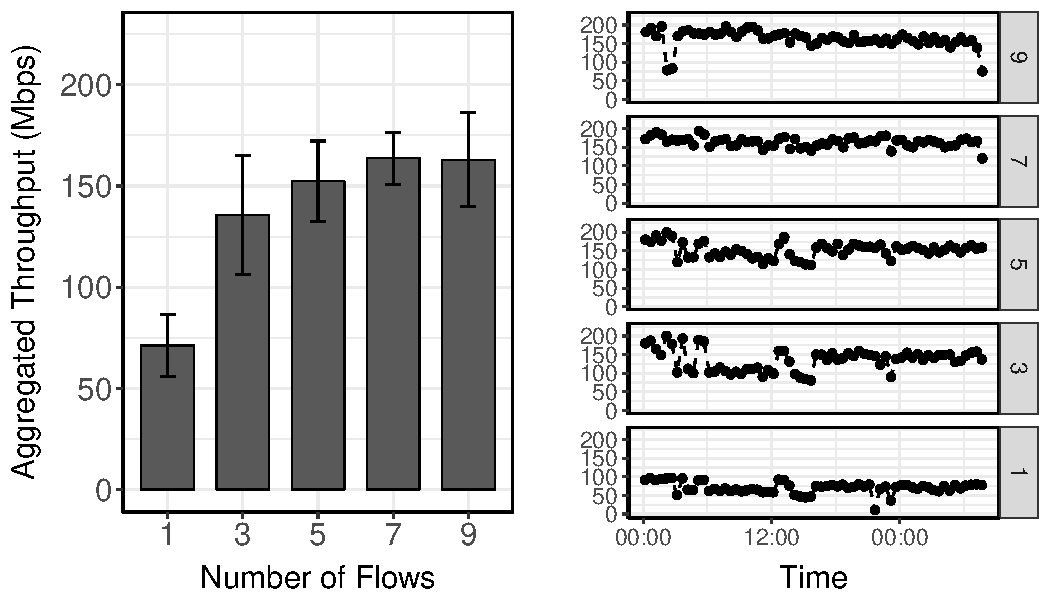
\includegraphics[width=.95\linewidth]{figures/motiv-aws.pdf}
  \caption{Bandwidth measurement between Amazon EC2 sites (from Ireland to
    California). Note the time-series plot has a resolution of 30 minutes.}
  \label{fig:bw}
\end{figure}

\begin{figure*}
  \centering
  \includegraphics[width=1.0\linewidth]{figures/motiv-app-specific.pdf}
  \caption{Application specific adaptations doesn't generalize. There are often
    multiple dimensions to explore. Degradation has different impact along
    different dimension}
  \label{fig:app-specific}
\end{figure*}

To understand the bandwidth characteristics in the wide-area, we conducted a
simple measurement using Amazon EC2. We use iPerf~\cite{iperf3} to measure the
pair-wise bandwidth between four geo-distributed sites throughout the day. We
observed large variance in the measured bandwidth and one such pair of sites is
shown in~\autoref{fig:bw}. Regardless of the number of flows\footnote{EC2 has a
  per-flow and per-VM rate limiting~\cite{zhang2016guaranteeing}.}, there exist
occasions when the available bandwidth is almost halved. We believe the
back-haul links between EC2 sites are better (if not at least representative) in
comparison to the general wide-area links. The varying nature poses real
challenge to the realization and successful deployment of wide-area streaming
applications.

Similar variations have also been reported in wireless
network~\cite{biswas2015large}, ISP network~\cite{grover2013peeking}, cellular
network~\cite{nikravesh2014mobile}.

% \begin{figure}
%   \centering
%   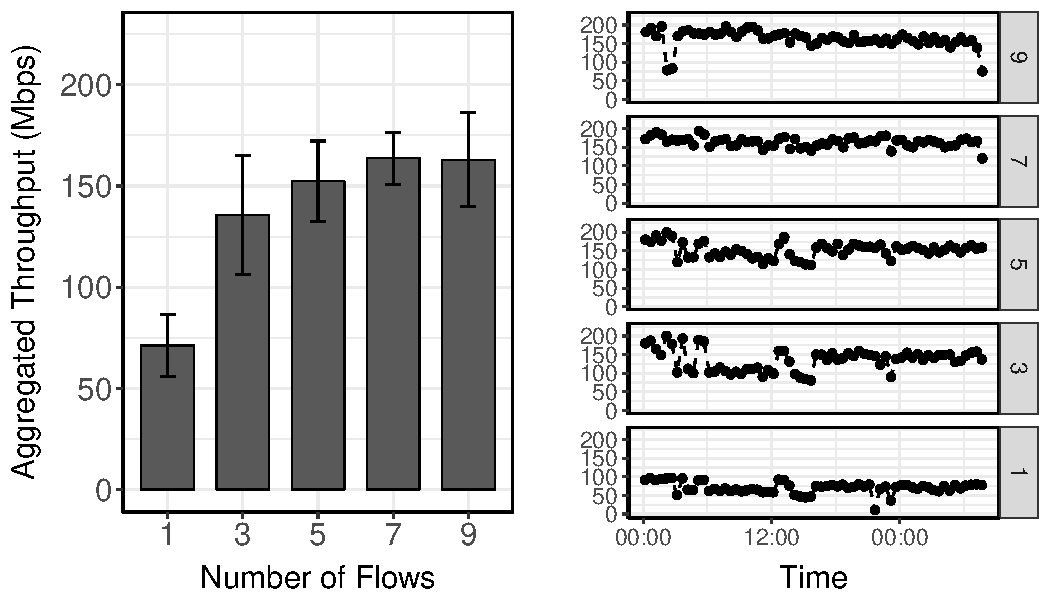
\includegraphics[width=.95\linewidth]{figures/motiv-aws.pdf}
%   \caption{Bandwidth measurement between Amazon EC2 sites (from Ireland to
%     California). Note the time-series plot has a resolution of 30 minutes.}
%   \label{fig:bw}
% \end{figure}

\subsection{Making the Case for a System Approach}
\label{sec:bat}

When facing insufficient resources, applications that do not adapt will suffer
severe performance penalty: such as a backlog of data for TCP or uncontrolled
packet loss for UDP. We argue that applications should be made adaptive to the
varying resource.

While adaptive streaming exist in certain application domain, there has not been
a general solution. Consider video streaming applications that have been
extensively studied in the literature. There are a plethora of encoding
techniques~\cite{richardson2011h, grange2016vp9} with adaptive
strategies~\cite{yin2015control, michalos2012dynamic, pantos2016http}, however,
their primary goal is to optimize end-user quality of experience (QoE).  When
end users consume a video clip, a smooth video is often more enjoyable than
videos with intermittent pauses, even though with crisp images.

Video streaming analytics often have different goals, therefore entail different
adaptive strategies. For example, many computer vision detection algorithms rely
on the edge information~\cite{canny1986computational, lowe2004distinctive,
  viola2001rapid} while object tracking applications works best when the
inter-frame difference is small~\cite{allen2004object}.

Further, even the same query, when used in different context, requires different
strategies. For example, pedestrian detection can be deployed with a ground
stationary camera. When taking pedestrian walking speed into consideration, it's
not necessary to guarantee a high frame rate. But because these surveillance
cameras are far from the target, it's crucial to have a high-resolution and
sharp image. On the other hand, when deployed with a mobile phone, due to the
movement of the camera, reducing frame rate will introduce significant
errors.

This motivates us to take a system-level approach that synthesize different
adaptation strategies for different queries and contexts.

%%% Local Variables:
%%% mode: latex
%%% TeX-master: "sosp17"
%%% End:
